\documentclass[a4paper,12pt,twocolumn]{extarticle}

\usepackage[T1]{fontenc}
\usepackage[utf8]{inputenc}
\usepackage{lmodern}

\usepackage[]{parskip}
\usepackage{hyperref, wrapfig, float, amsmath, adjustbox, array, pdflscape, soul, color, extsizes}
\usepackage{booktabs}
\usepackage{lscape}

\renewcommand{\arraystretch}{2}
\renewcommand{\contentsname}{Spis treści}
\renewcommand{\refname}{Bibliografia}
\renewcommand{\figurename}{Rys.}
\renewcommand{\tablename}{Tab.}

\usepackage{geometry}
\geometry{
  a4paper,
  margin=30mm,
  bottom=30mm
}

\usepackage{graphicx}
\usepackage[font=footnotesize,labelfont=bf,justification=centering]{caption}
\usepackage{subcaption}
\graphicspath{ {./images/}{../images/} }

\newcommand{\mathcolorbox}[1]{
  \begin{center}
    \colorbox{yellow}{$\displaystyle #1$}
  \end{center}
}
\newcommand{\pvec}[1]{
  \vec{#1}\mkern2mu\vphantom{#1}
}
\newcommand{\angstrom}{\mbox{\normalfont\AA}}

\begin{document}
  \onecolumn
  \begin{titlepage}
    \begin{center}
      \begin{figure}[H]
        \centering
        
\includegraphics[scale=.125]{logopp.png}
      \end{figure}
      \vspace*{.05\textheight}
      \huge\textbf{Politechnika Poznańska}\\
      \large\textbf{Wydział Inżynierii Materiałowej i Fizyki Technicznej}\\
      \large\textbf{Fizyka Techniczna}\\
      \vspace*{.2\textheight}
      \huge\textbf{Sprawozdanie --- laboratorium LFM}\\
      \vspace*{.025\textheight}
      \large\textbf{Jakub Bąbelek\\(nr.\ albumu: 136454)}
    \end{center}
  \end{titlepage}

  \tableofcontents
  
  \clearpage
  \twocolumn

  \section{Wstęp}
  \subsection{Tarcie}
  Tarcie to siła towarzysząca przemieszczaniu się względem siebie dwóch ciał fizycznych,
  stykających się ze sobą oraz elementów tego samego ciała (tarcie wewnętrzne).

  Siła tarcia statycznego --- działająca kiedy ciała względem siebie pozostają w spoczynku ---
  równoważy siłę wypadkową wszystkich sił działających na ciało. Siła tarcia ma ten
  sam kierunek lecz przeciwny zwrot co siła wypadkowa. Za pomocą wzoru (\ref{eq:fr_static}),
  możemy określić maksymalną wartość siły tarcia.

  \begin{equation}
    T_s = \mu N
    \label{eq:fr_static}
  \end{equation}

  Jeżeli ciała względem siebie poruszają się, mamy do czynienia z siła tarcia
  dynamicznego, ma ona kierunek zgodny z ruchem ciała lecz przeciwny zwrot.
  Korzystając ze wzoru (\ref{eq:fr_dyn}) możemy obliczyć jej wartość.

  \begin{equation}
    T_d = \mu N
    \label{eq:fr_dyn}
  \end{equation}

  \begin{center}
    \tiny{
    gdzie: \( \mu\ -\ współczynnik\ tarcia,\ N\ -\ Siła\ nacisku \)
    }
  \end{center}

  Prawa tarcia:
  \begin{enumerate}
    \item{
      ``Siła tarcia ślizgowego między dwoma ciałami jest proporcjonalna do
      składowej normalnej siły utrzymującej ciała w zetknięciu (\ref{eq:fr}).''
      \begin{equation}
        T = \mu N
        \label{eq:fr}
      \end{equation}
    }
    \item ``Siła tarcia ślizgowego nie zależy od wielkości powierzchni zetknięcia ciał.''
    \item ``Z chwilą wprowadzenia ciała w ruch, siła tarcia nie zależy od prędkości.''
  \end{enumerate}

  \subsection{Tribologia}
  Tribologia to nauka badająca oddziaływanie ze sobą powierzchni ciał będących
  w ruchu względem siebie tj.\ takie zjawiska jak \textit{tarcie, smarowanie czy ścieranie}.
  Jest to dziedzina wysoce interdyscyplinarna, wykorzystuje wiedzę z wielu gałęzi nauki
  m.in. \textit{fizyki, chemii, materiałoznawstwa, matematyki, biologii oraz inżynierii}.

  Choć dziedzina ta nazwana została stosunkowo niedawno to pierwsze wzmianki na
  temat badań tarcia pomiędzy ciałami sięgają roku 1493. \textit{Leonardo da Vinci}
  jako pierwszy spisał podstawowe prawa dotyczące tarcia.

  \begin{figure}[H]
    \centering
    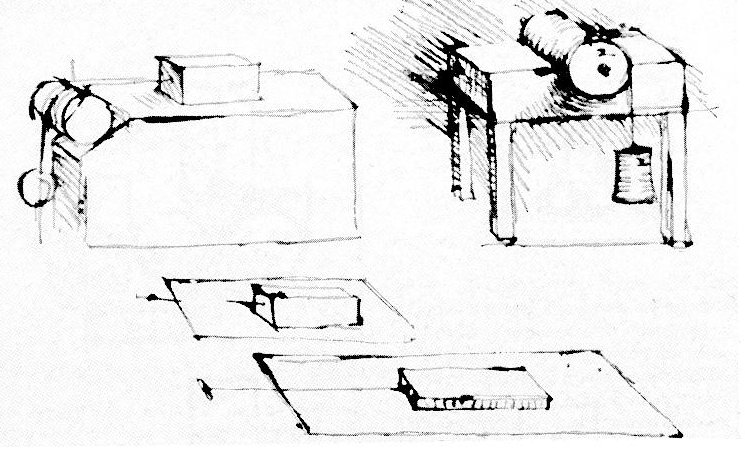
\includegraphics[width=.4\textwidth]{davinci.jpg}
    \caption{Szkice Leonarda da Vinci dot.\ przeprowadzanych przez niego eksperymentów}
    \label{fig:davinci}
  \end{figure}

  Termin \textit{tribologia} został spopularyzowany po opublikowaniu po opublikowaniu
  w 1966 przez Petera Josta pracy traktującej o wpływie tarcia, ścierania i korozji
  materiałów na ekonomię Wielkiej Brytanii.

  \clearpage
  \section{Zależność siły tarcia od siły nacisku dla \( Au-SiO_x \) oraz \( SiO_x-SiO_x \)}
  Za pomocą programu AtomicJ eksportowałem dane do programu MS Office Excel a
  następnie dokonałem analizy siły tarcia dla badanych wartości siły nacisku
  (\figurename~\ref{fig:wykres}).

  Następnie używając metody regresji liniowej odczytałem wartości współczynnika
  tarcia kinetycznego dla obu powierzchni (\tablename~\ref{tab:kin_fr}).

  \begin{table}[H]
    \centering
    \begin{adjustbox}{max width = .5\textwidth}
      \begin{tabular}{cc}
      \toprule
      \textbf{Powierzchnie} & \textbf{Wsp.\ tarcia kinetycznego} \\
      \midrule
      \( Au-SiO_x \)        & 0.282                              \\
      \( SiO_x-SiO_x \)     & 0.311                              \\
      \bottomrule
      \end{tabular}
    \end{adjustbox}
    \caption{Wsp. tarcia kinetycznego dla obu powierzchni}
    \label{tab:kin_fr}
  \end{table}

  Wykonałem również histogramy siły tarcia w kierunku pierwotnym i powrotnym dla
  siły nacisku 20nN oraz pierwotnym dla 40nN i 120nN

  \begin{figure}[H]
    \centering
    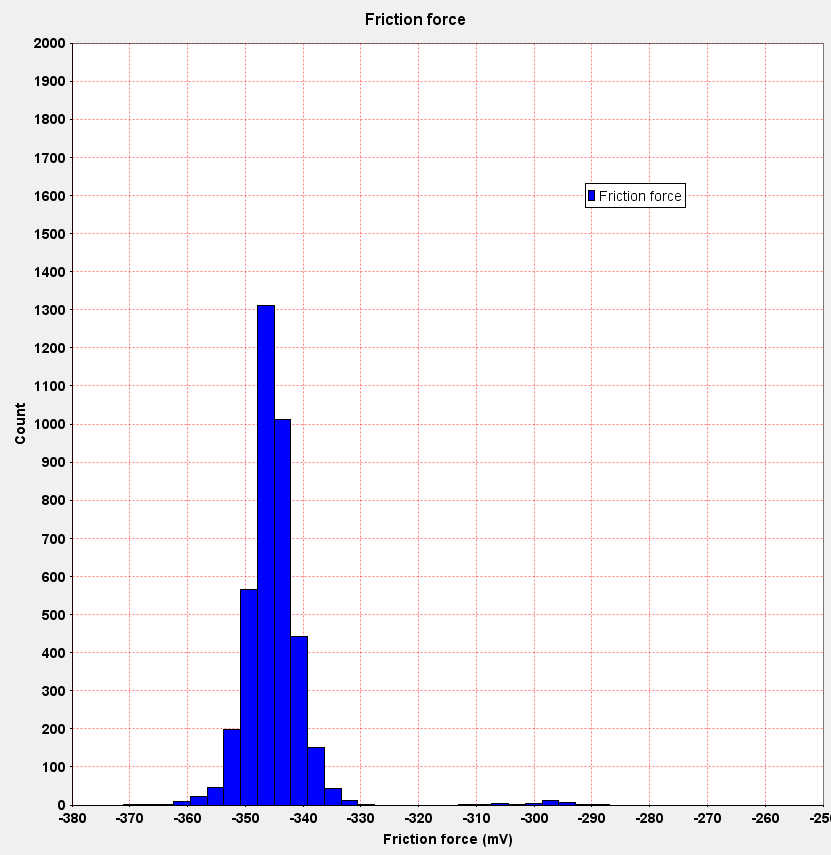
\includegraphics[width=.35\textwidth]{10fwd.png}
    \caption{Histogram dla 20nN\\kierunek pierwotny}
    \label{fig:10fwd}
  \end{figure}
  \begin{figure}[H]
    \centering
    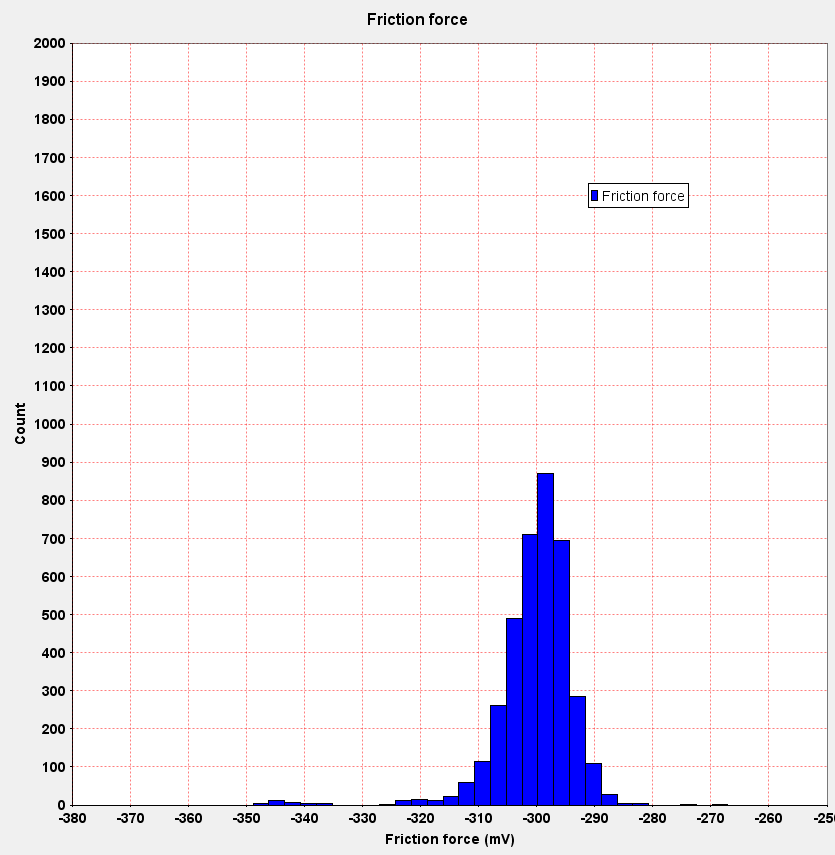
\includegraphics[width=.35\textwidth]{10bwd.png}
    \caption{Histogram dla 20nN\\kierunek powrotny}
    \label{fig:10bwd}
  \end{figure}
  \begin{figure}[H]
    \centering
    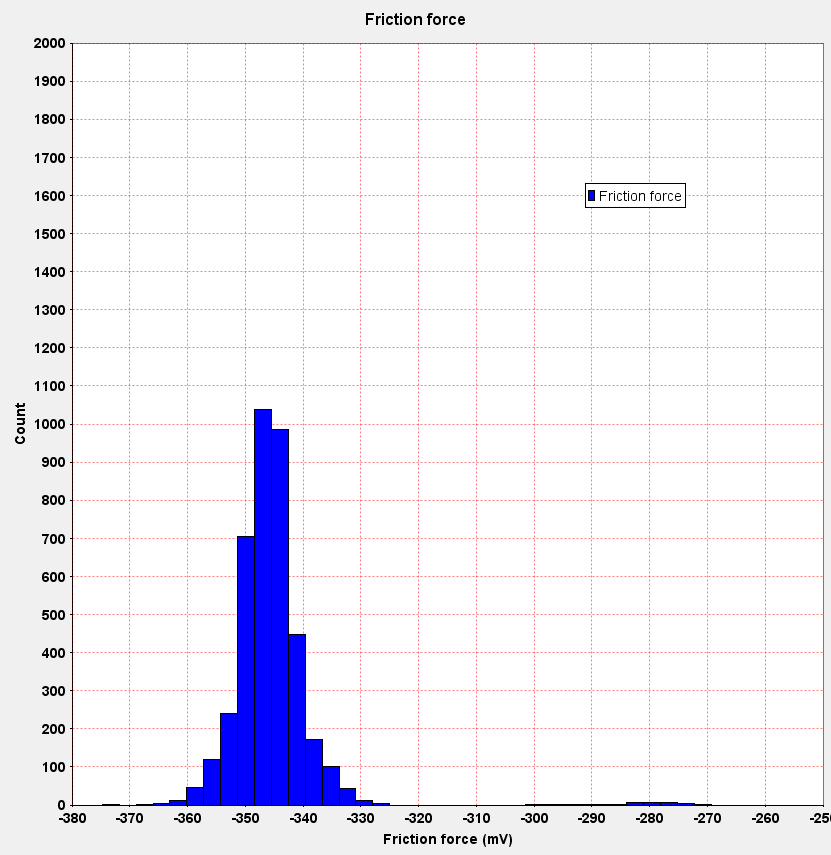
\includegraphics[width=.35\textwidth]{20fwd.png}
    \caption{Histogram dla 40nN\\kierunek pierwotny}
    \label{fig:20fwd}
  \end{figure}
  \begin{figure}[b]
    \centering
    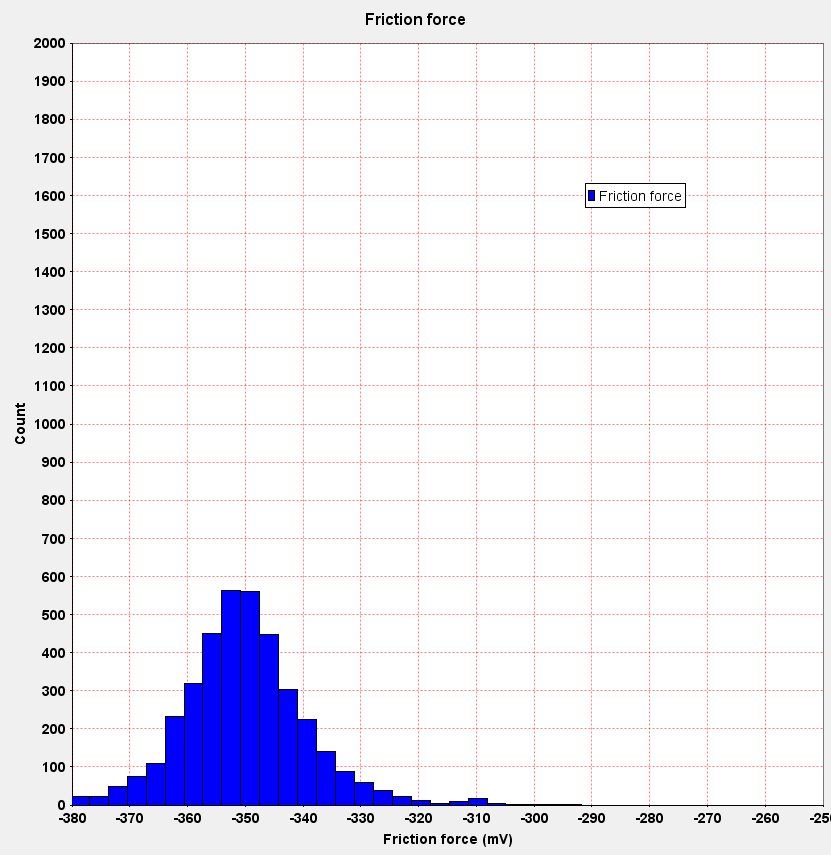
\includegraphics[width=.35\textwidth]{60fwd.png}
    \caption{Histogram dla 120nN\\kierunek pierwotny}
    \label{fig:60fwd}
  \end{figure}

  \clearpage
  \onecolumn
  \begin{landscape}
    \begin{figure}
      \centering
      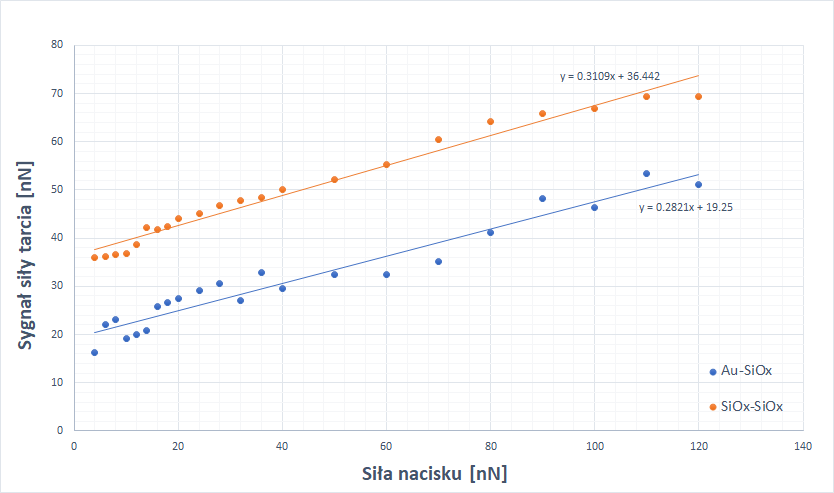
\includegraphics[width=22.5cm]{wykres.png}
      \caption{Wykres zależności siły tarcia od siły nacisku.}
      \label{fig:wykres}
    \end{figure}
  \end{landscape}
  \twocolumn
  \clearpage

  \section{Obrazy topografii \( Au-SiO_x \)}

  Aby uzyskać obraz topografii poddałem dane obróbce w programie Gwyddion.
  Po użyciu funkcji \textit{Align rows} oraz usunięciu ``artefaktów'' obrazu
  objawiających się w formie poziomych ``cieni'' widocznych na obrazie topografii
  uzyskałem następujące obrazy.

  \begin{figure}[H]
    \centering
    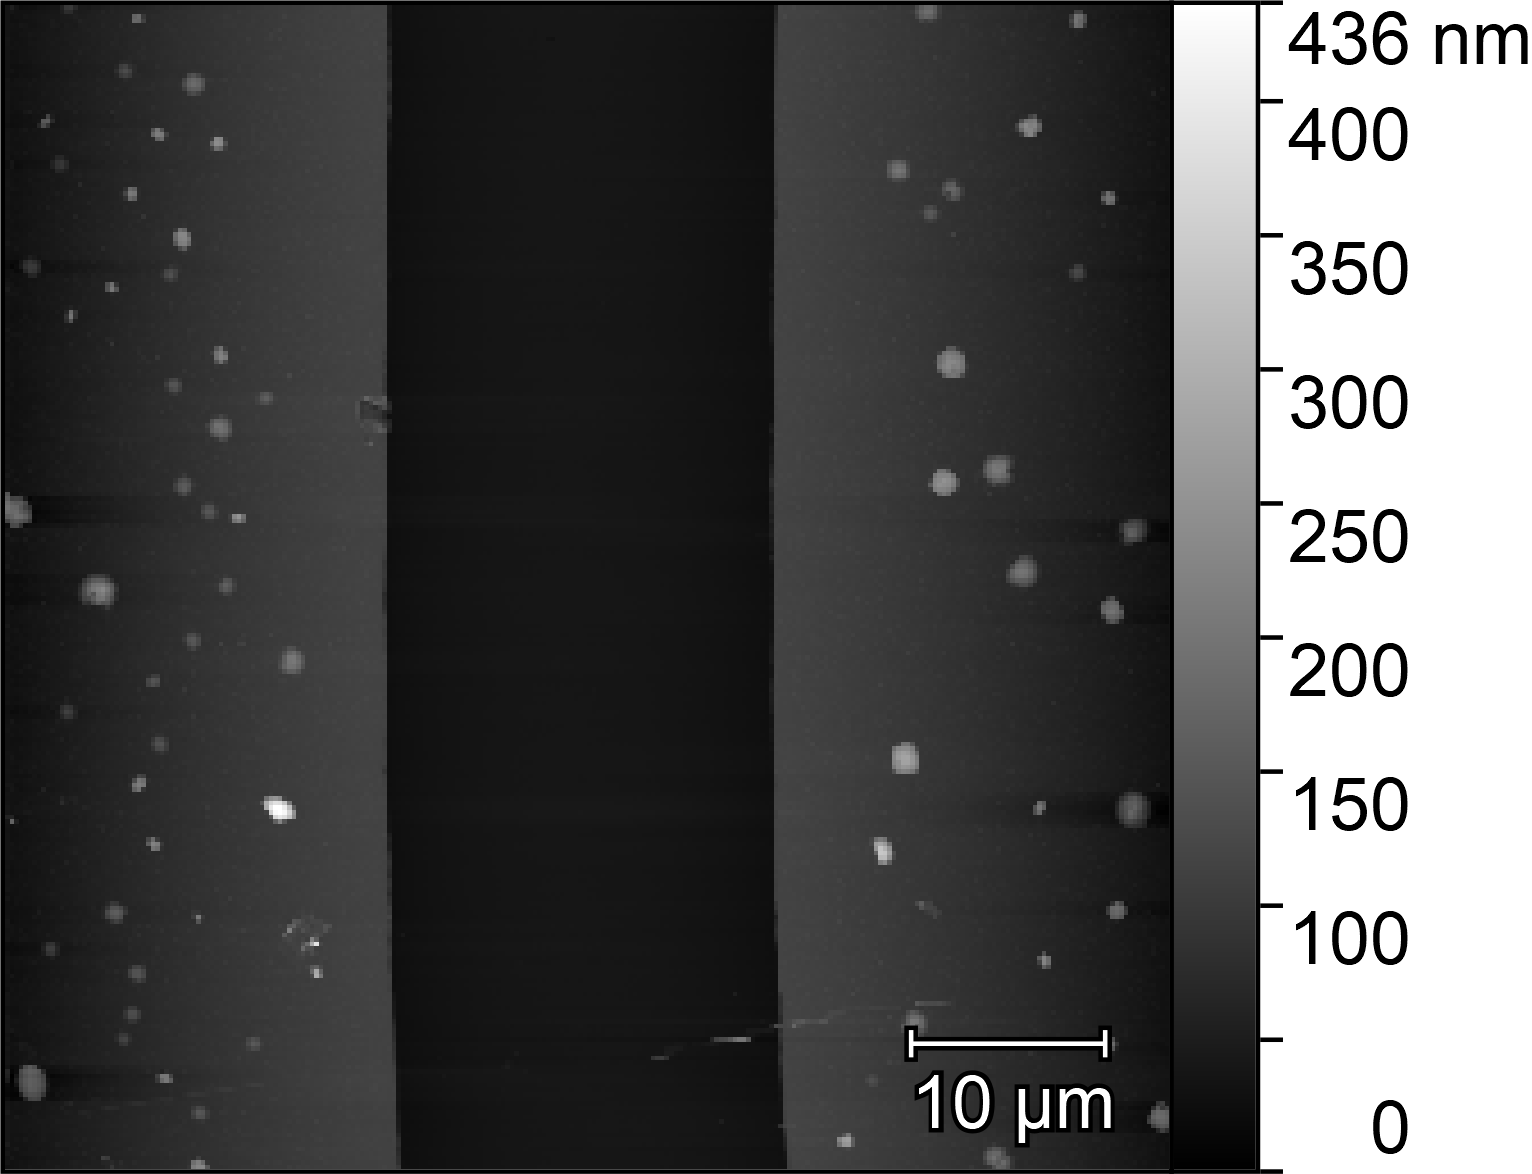
\includegraphics[width=.5\textwidth]{ausi_topo.png}
    \caption{Topografia po obróbce w programie Gwyddion}
    \label{fig:ausi_topo}
  \end{figure}

  Z obrazu przekroju (\figurename~\ref{fig:ausi_przekroj}) możemy odczytać
  szerokość paska tlenku krzemu która wynosi \(19.85\mu m\)

  \begin{figure}[H]
    \centering
    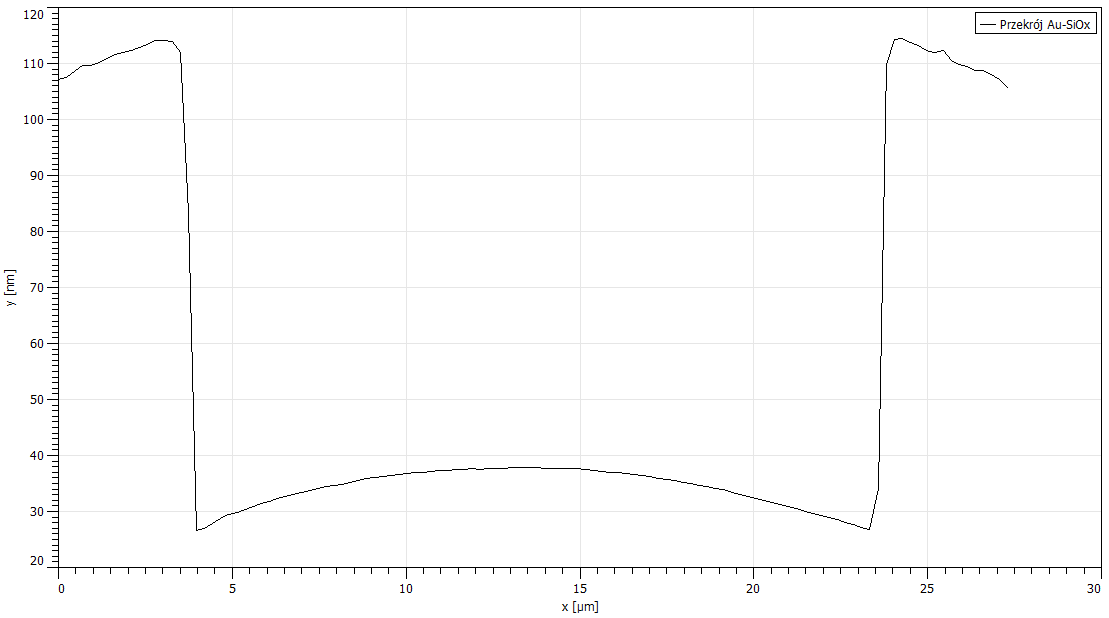
\includegraphics[width=.5\textwidth]{ausi_przekroj.png}
    \caption{Przekrój obrazu topografii}
    \label{fig:ausi_przekroj}
  \end{figure}
  \begin{figure}[H]
    \centering
    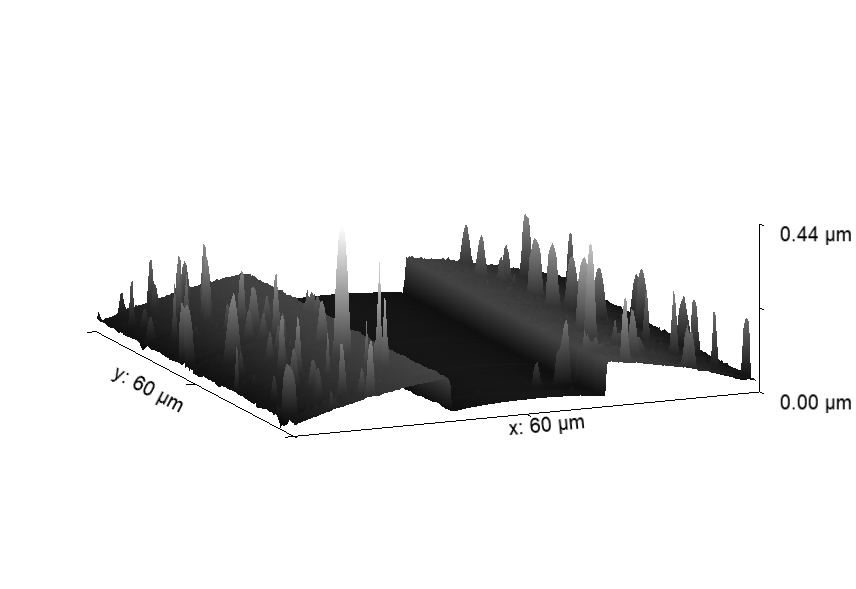
\includegraphics[width=.5\textwidth]{ausi_3d.png}
    \caption{Topografia --- widok 3d}
    \label{fig:ausi_3d}
  \end{figure}

  \clearpage
  \section{Obrazy płyt DVD oraz HD DVD}
  Ilość danych jakie możemy zapisać na płycie zależy od gęstości w jakiej znaleźć
  się one mogą na jej powierzchni, analiza danych z mikroskopu pozwala na obliczenie
  z jaką gęstością możliwy jest zapis na obu nośnikach.

  \subsection{DVD}

  \begin{figure}[H]
    \centering
    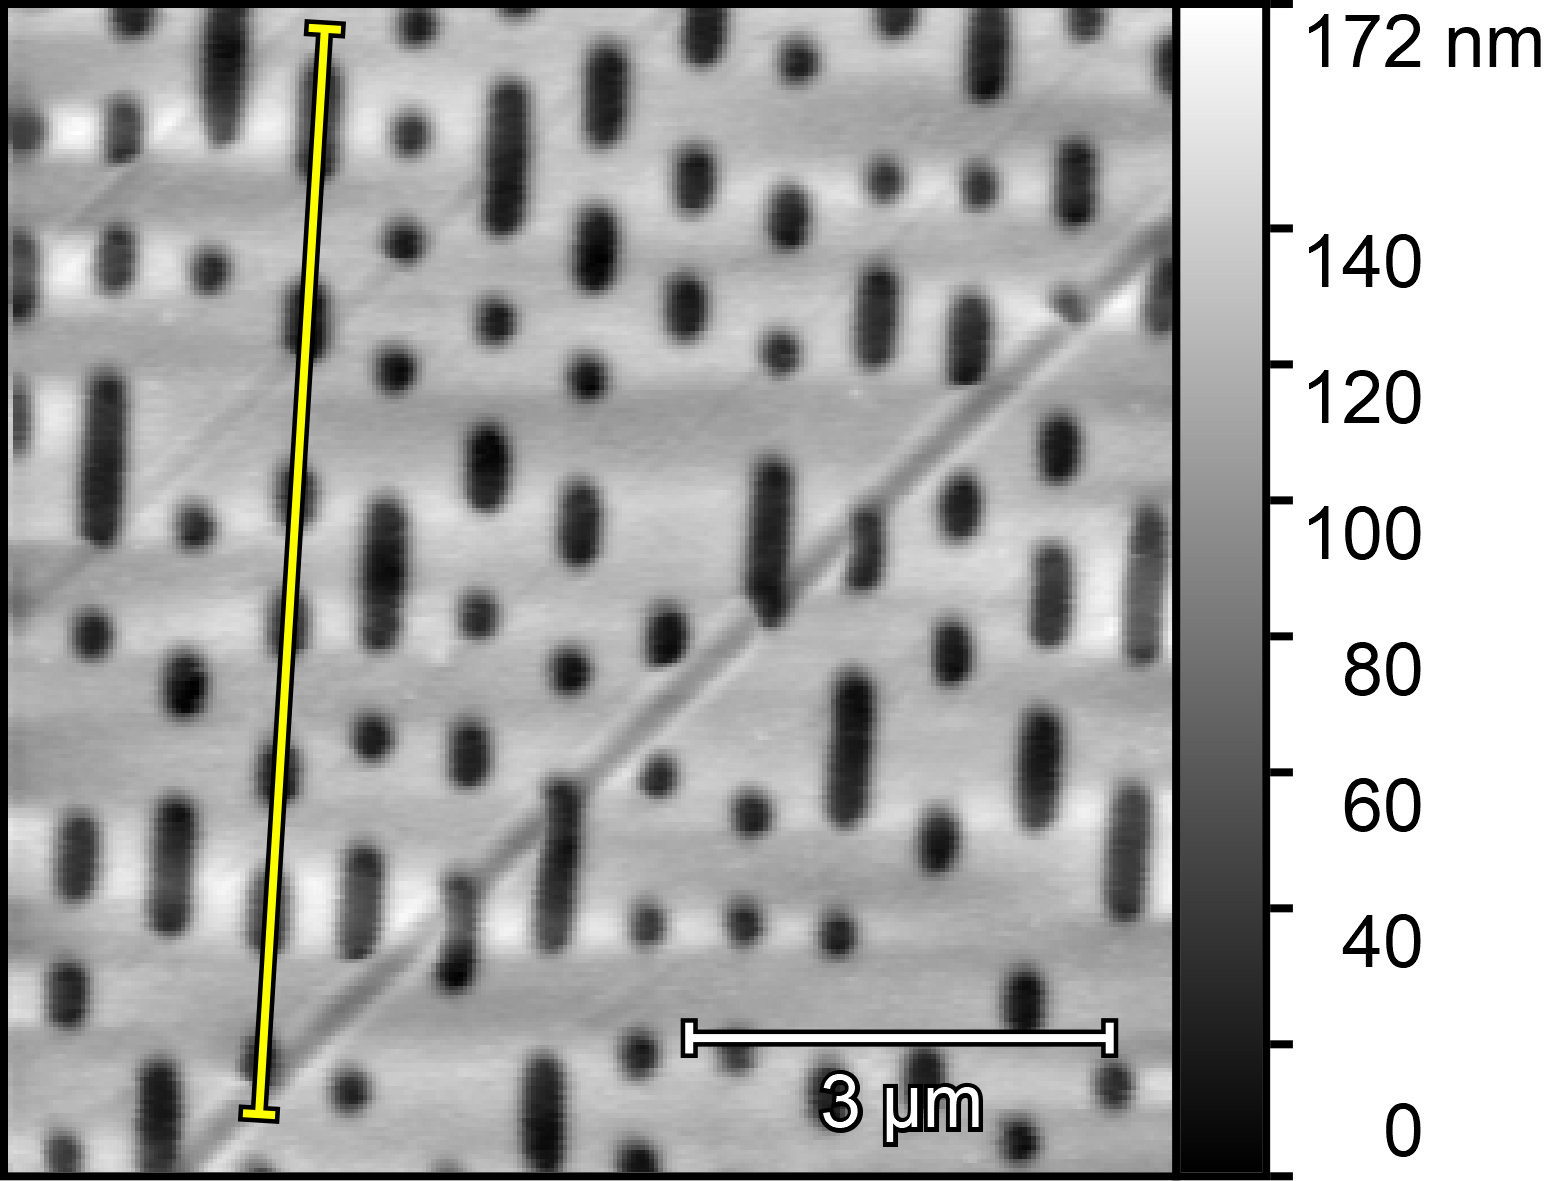
\includegraphics[width=.4\textwidth]{dvd_topo.png}
    \caption{Topografia płyty DVD}
    \label{fig:dvd_topo}
  \end{figure}

  \begin{figure}[H]
    \centering
    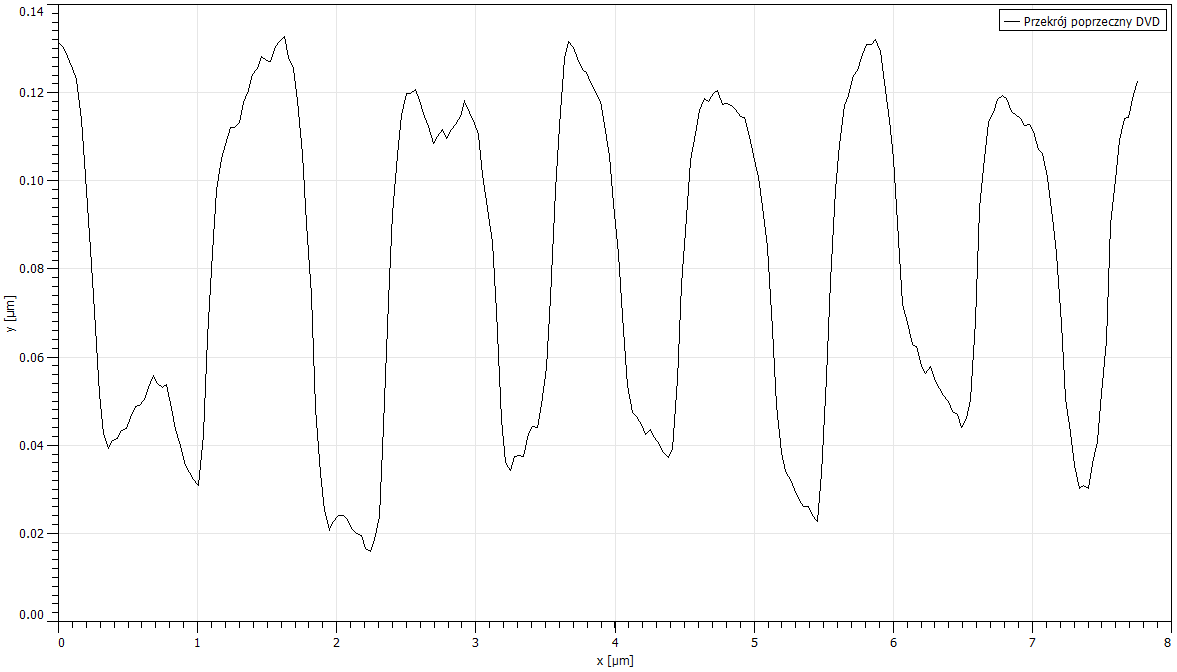
\includegraphics[width=.4\textwidth]{dvd_przekroj.png}
    \caption{Przekrój płyty DVD}
    \label{fig:dvd_przekroj}
  \end{figure}

  Zaznaczając maską wszystkie rowki (\figurename~\ref{fig:dvd_grains}) na
  płycie dvd i używając funkcji \textit{Grains summary} możemy policzyć ich
  ilość która wynosi 90

  \begin{figure}[H]
    \centering
    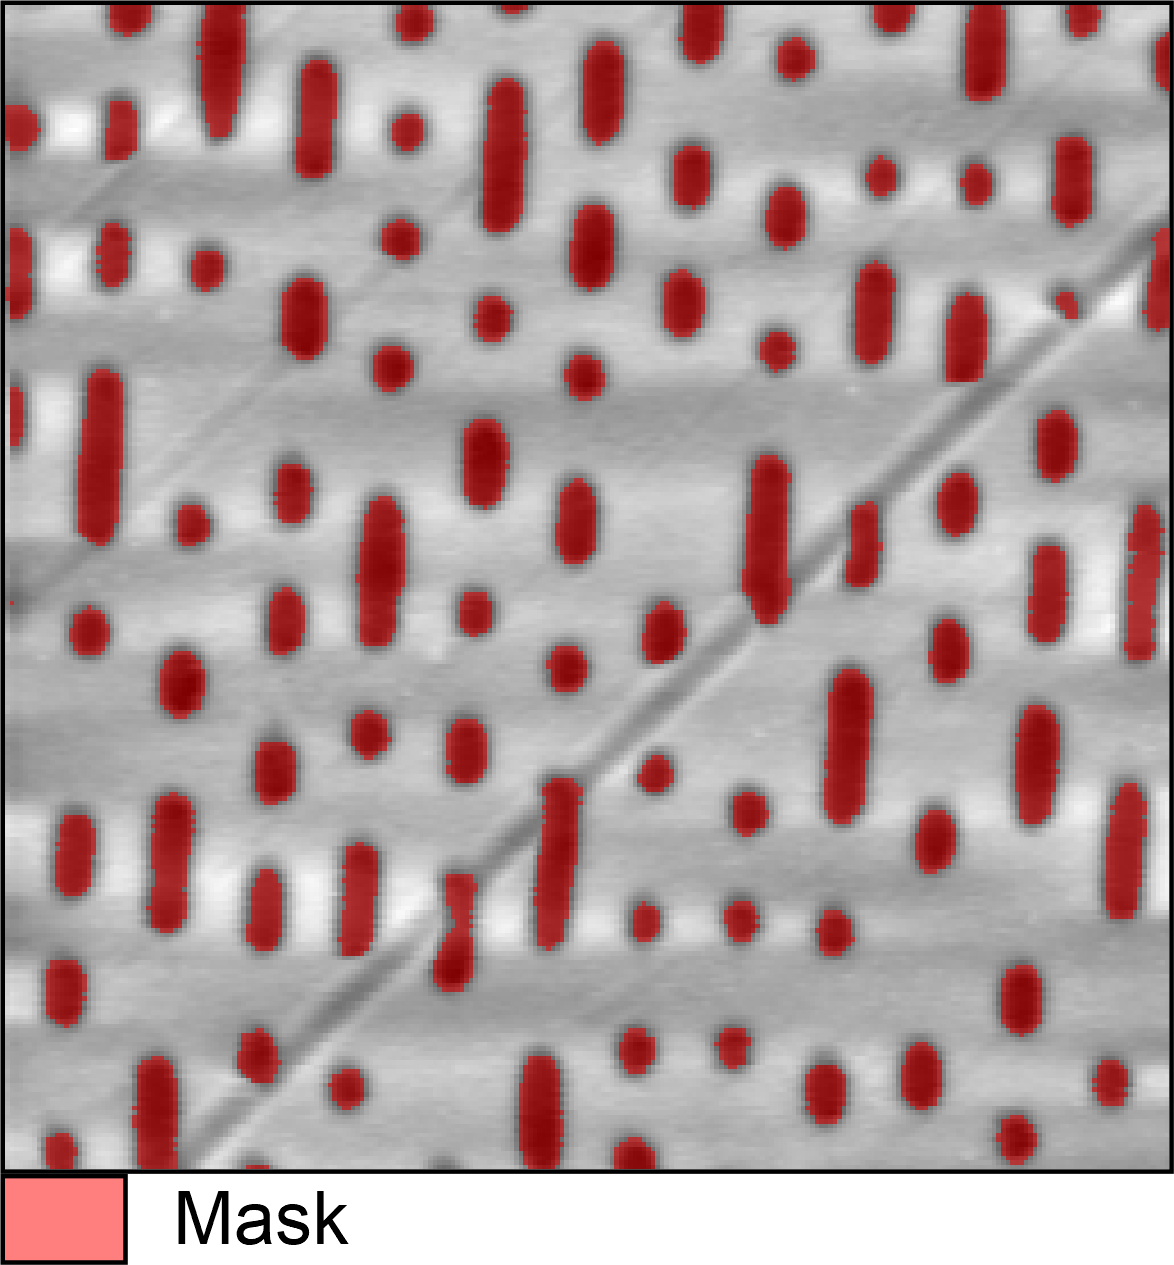
\includegraphics[width=.4\textwidth]{dvd_grains.png}
    \caption{Obraz po zaznaczeniu rowków dla płyty DVD}
    \label{fig:dvd_grains}
  \end{figure}

  \subsection{HD DVD}
  Wszystkie powyższe czynności zostały powtórzone dla płyty HD DVD

  \begin{figure}[H]
    \centering
    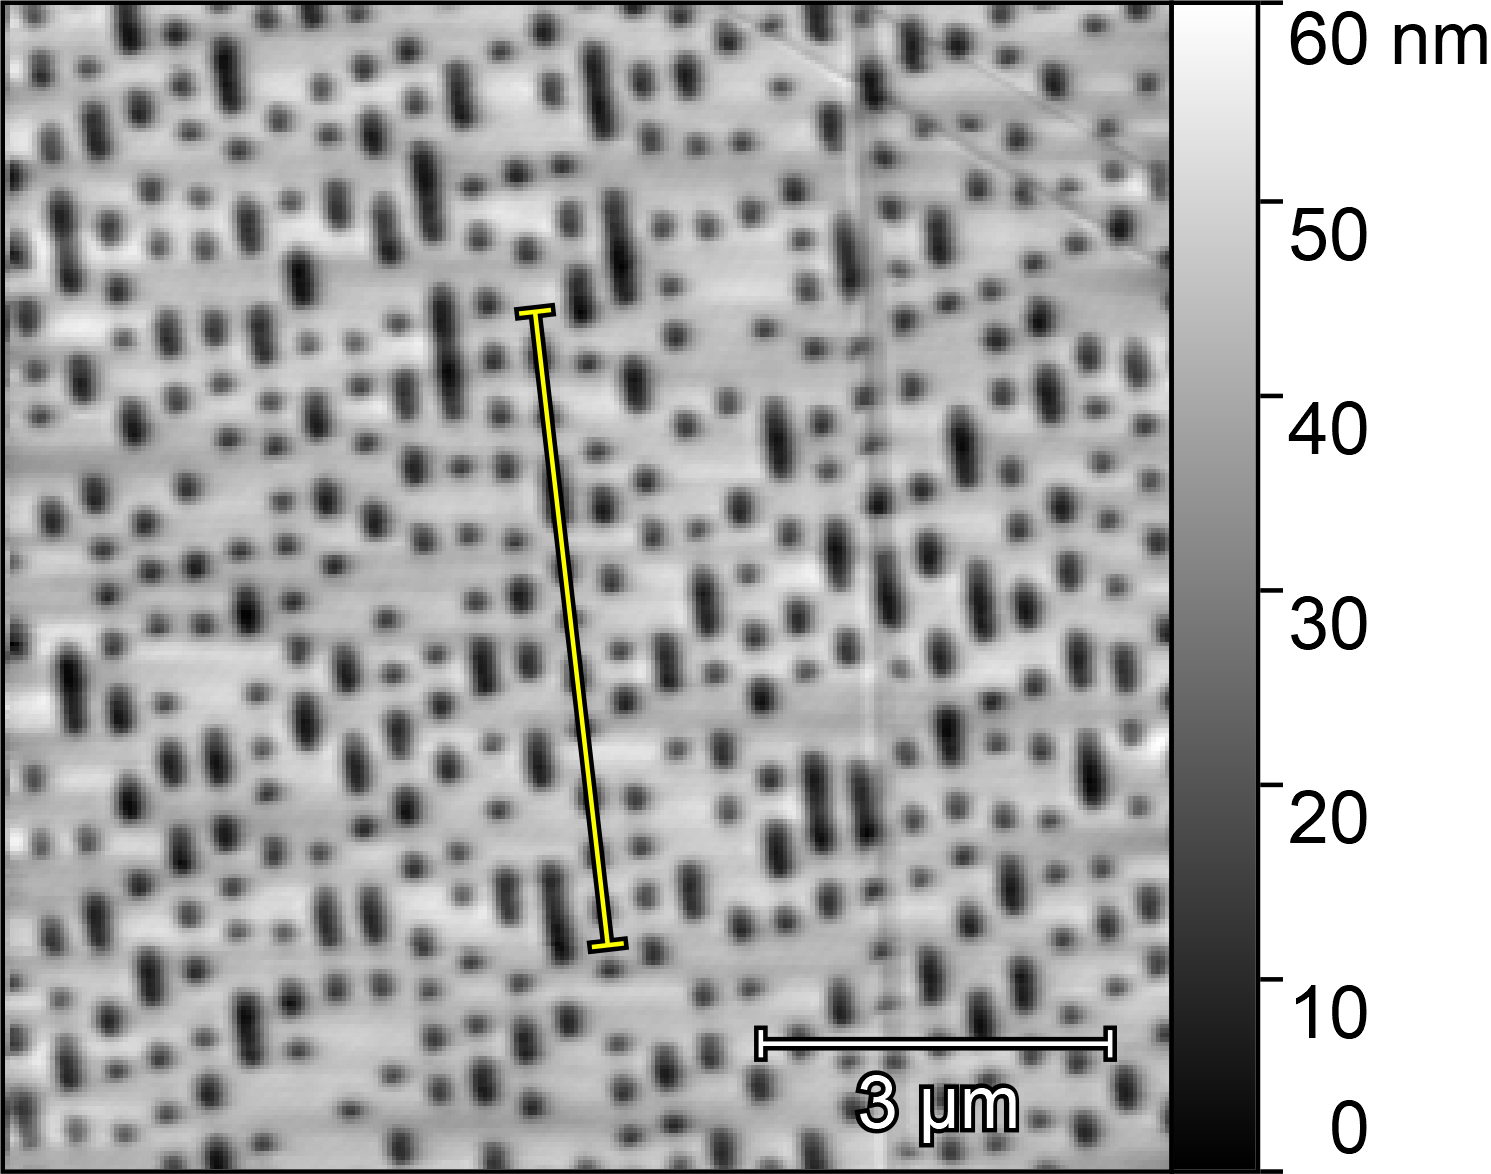
\includegraphics[width=.4\textwidth]{hddvd_topo.png}
    \caption{Topografia płyty HD DVD}
    \label{fig:hddvd_topo}
  \end{figure}

  \begin{figure}[H]
    \centering
    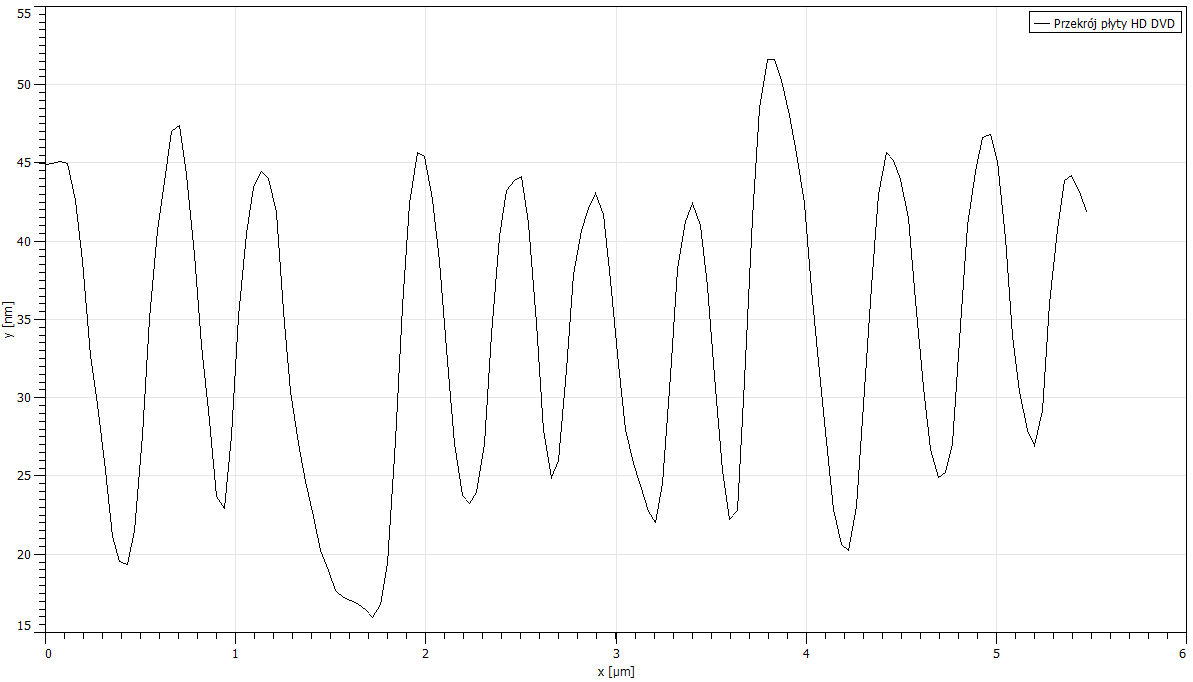
\includegraphics[width=.4\textwidth]{hddvd_przekroj.png}
    \caption{Przekrój płyty HD DVD}
    \label{fig:hddvd_przekroj}
  \end{figure}

  \begin{figure}[H]
    \centering
    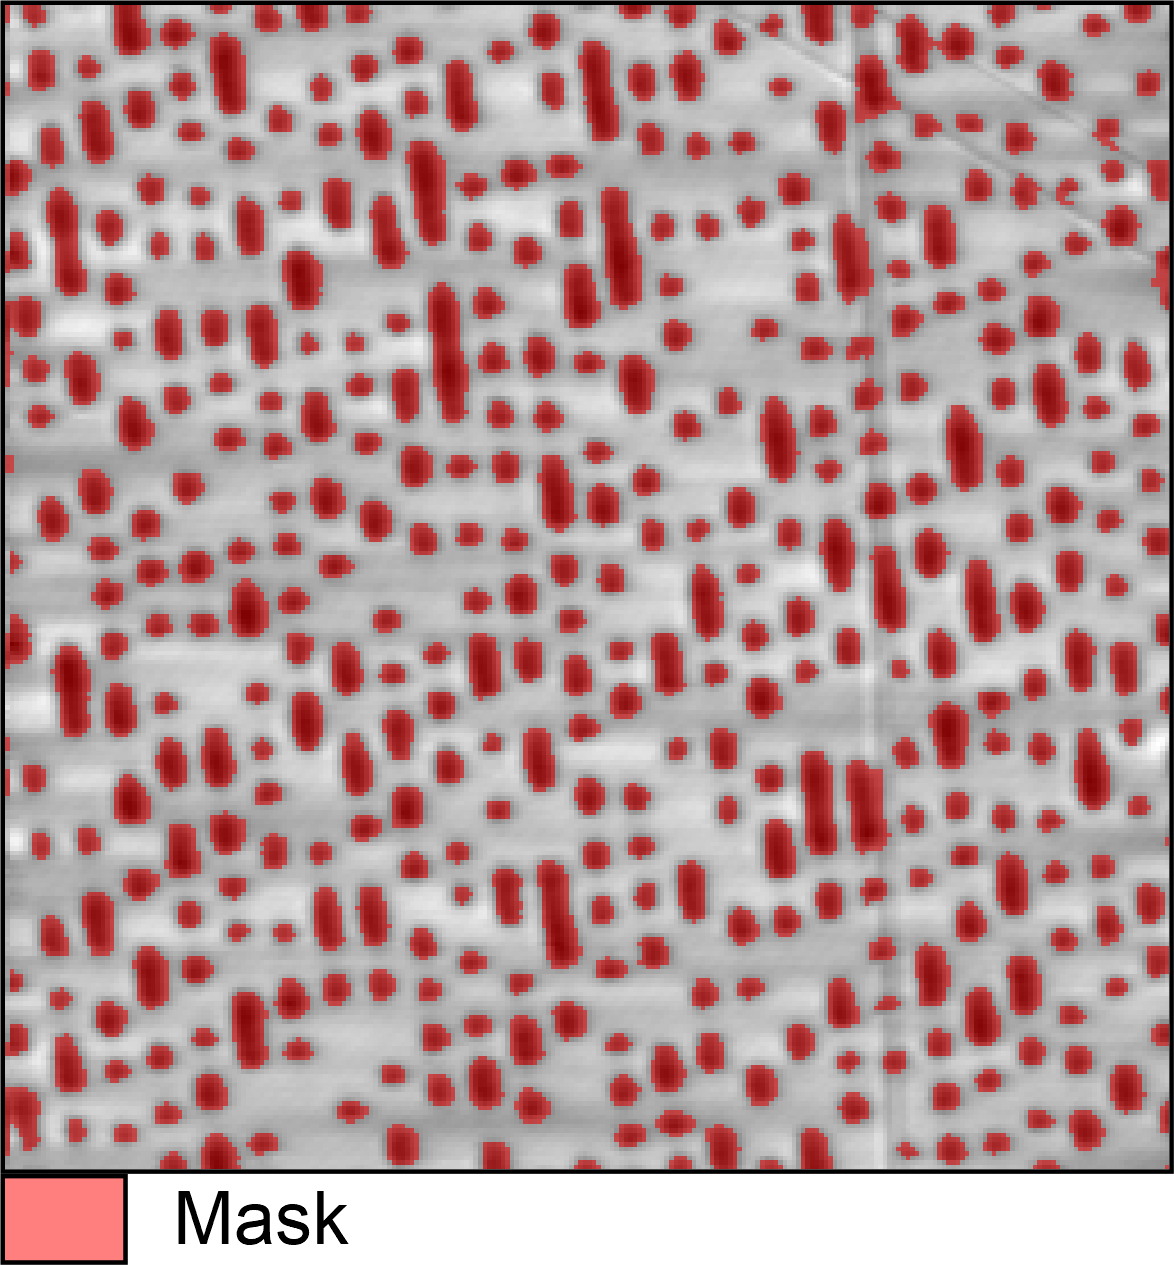
\includegraphics[width=.4\textwidth]{hddvd_grains.png}
    \caption{Obraz po zaznaczeniu rowków dla płyty HD DVD}
    \label{fig:hddvd_grains}
  \end{figure}

  \begin{table}[H]
    \centering
    \begin{adjustbox}{max width = .5\textwidth}
      \begin{tabular}{cc}
        \toprule
        \textbf{Nośnik}   & \textbf{Liczba rowków} \\
        \midrule
        DVD               & 90                     \\
        HD DVD            & 280                    \\
        \midrule
        \textbf{Stosunek} & 3.11                   \\
        \bottomrule
      \end{tabular}
    \end{adjustbox}
    \caption{Liczba rowków na obu płytach}
    \label{tab:grain_num}
  \end{table}

  \clearpage

  \section{Topografia i sygnał tarcia siatki kalibracyjnej}
  \begin{figure}[H]
    \centering
    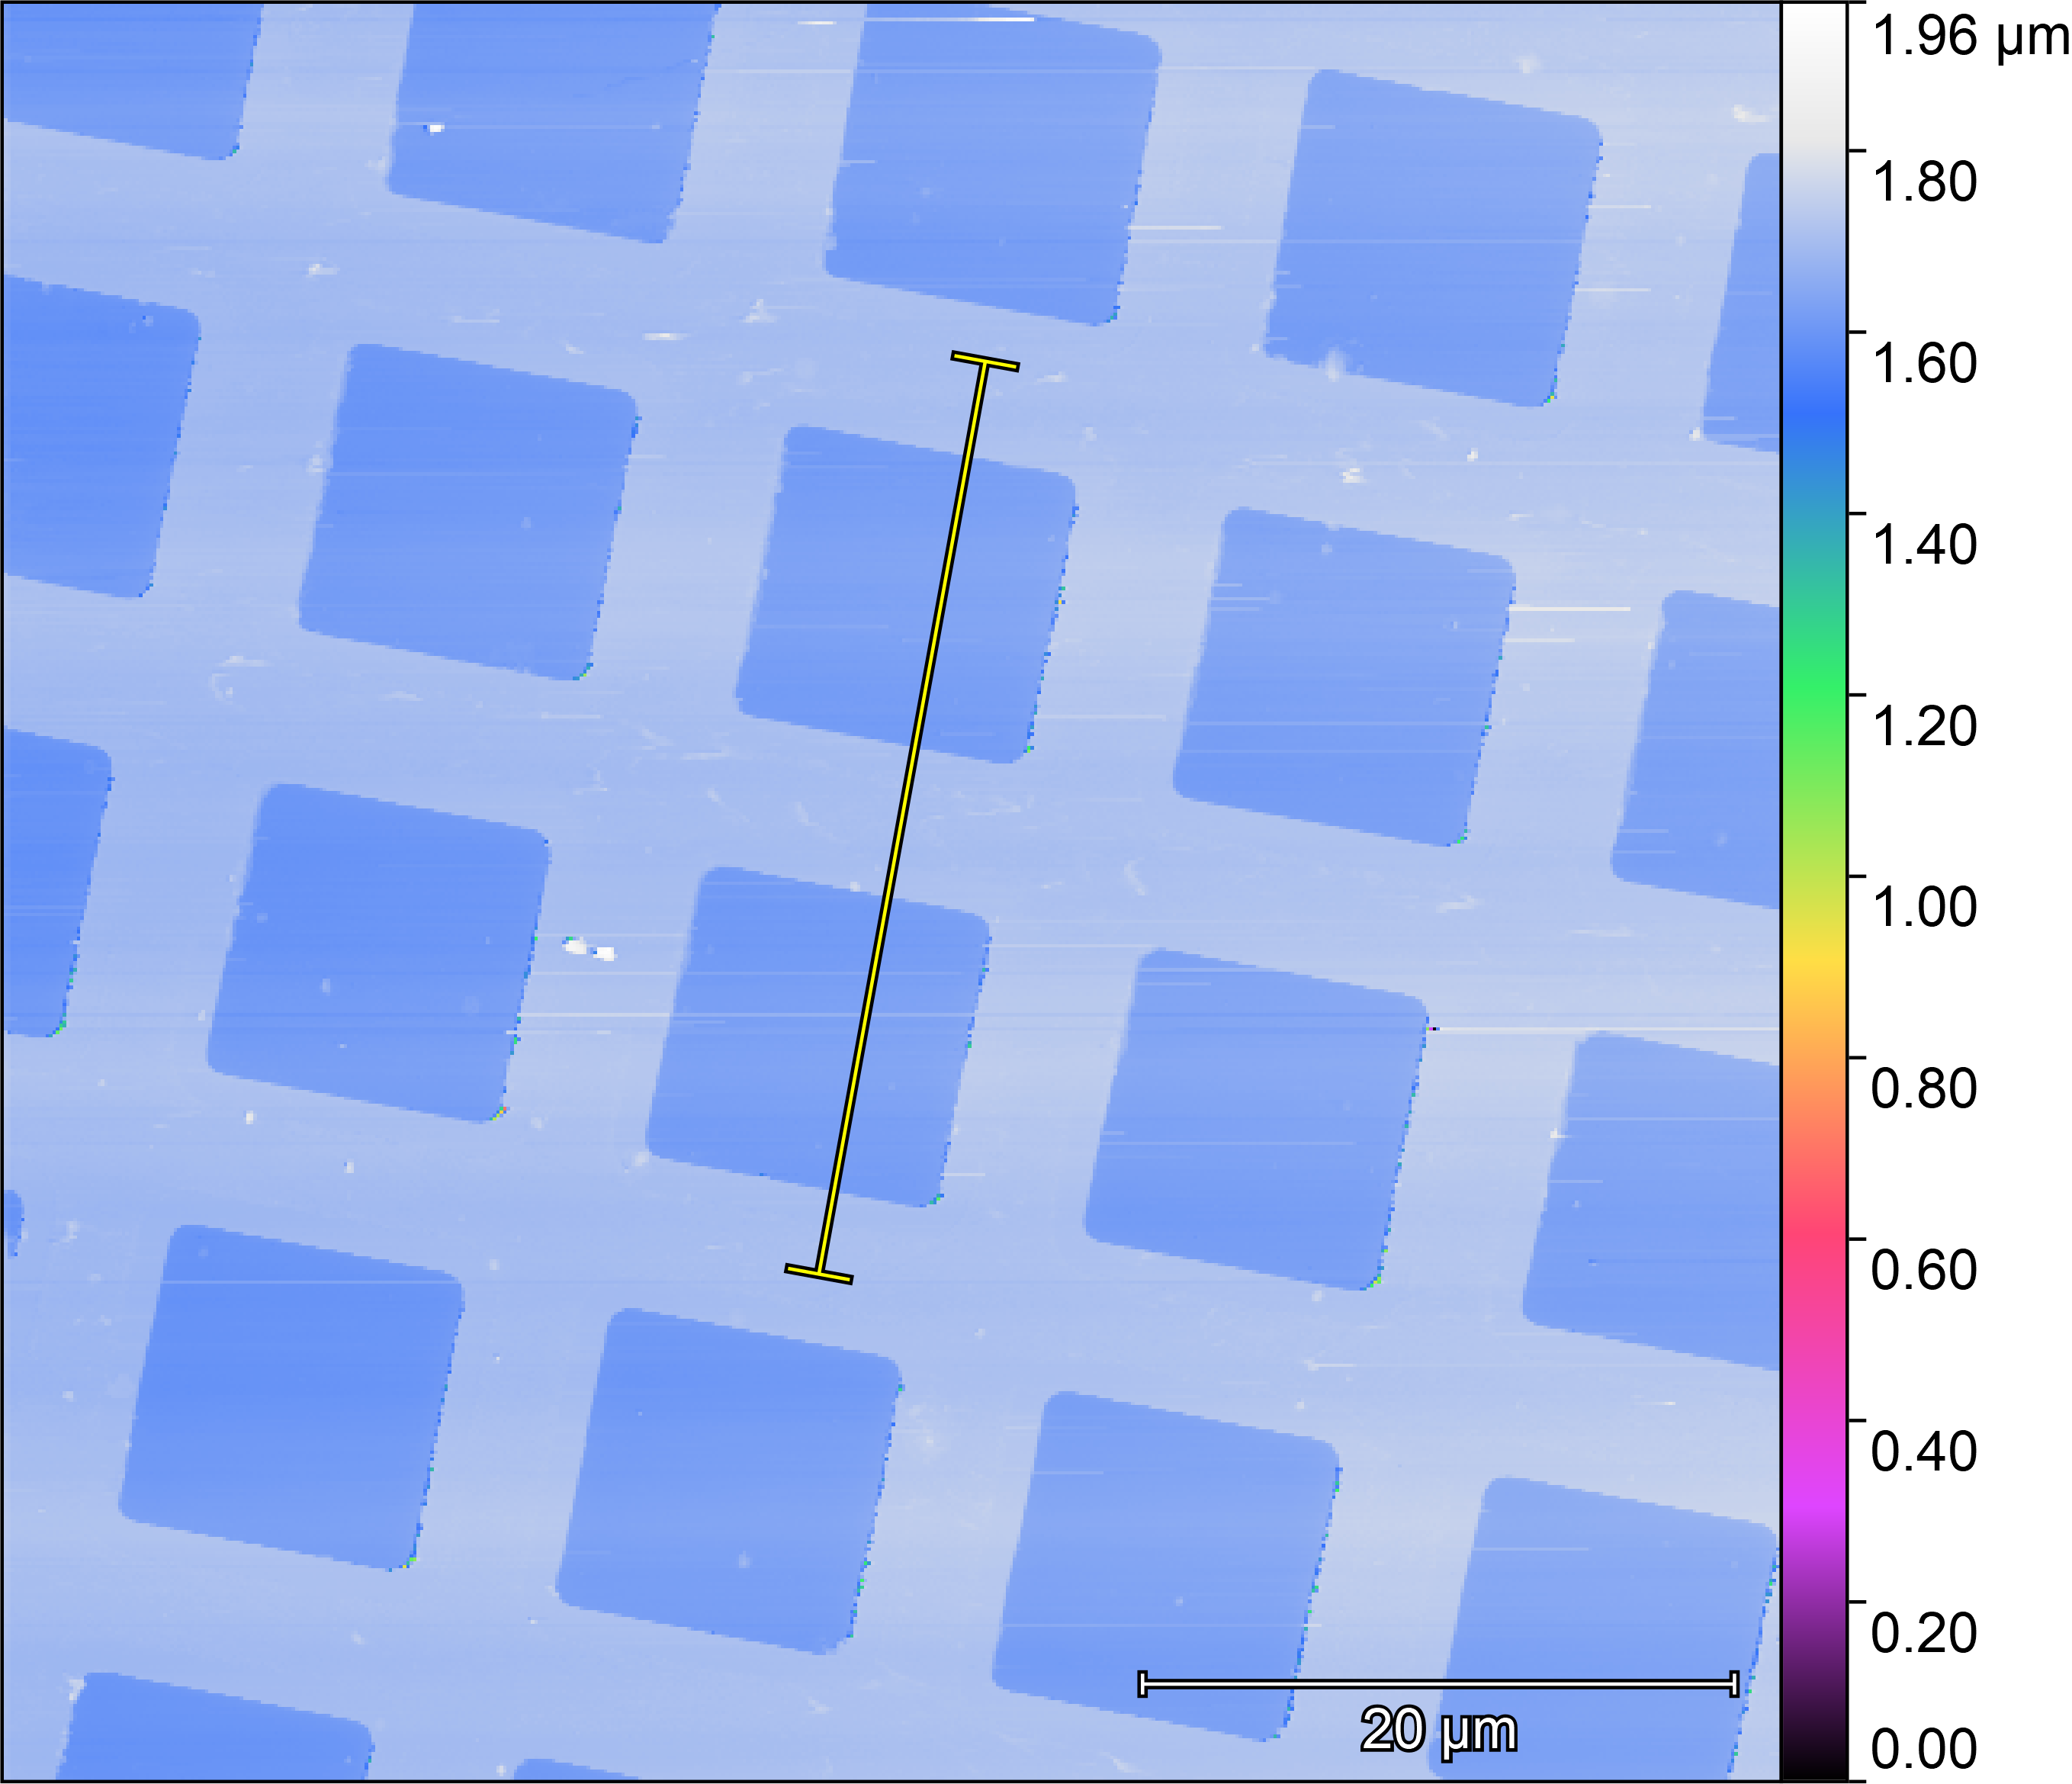
\includegraphics[width=.4\textwidth]{siatka_topo.png}
    \caption{Topografia siatki kalibracyjnej}
    \label{fig:siatka_topo}
  \end{figure}
  \begin{figure}[H]
    \centering
    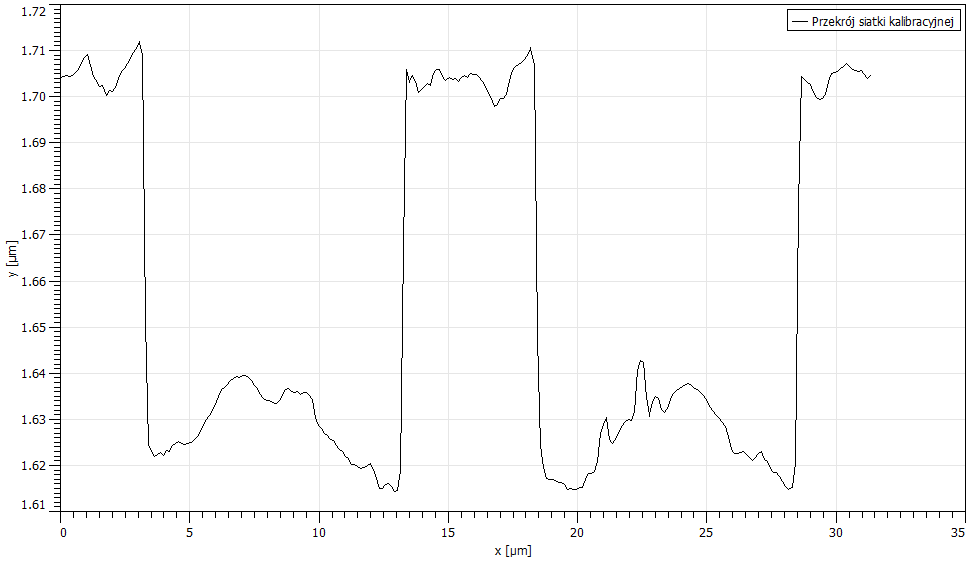
\includegraphics[width=.4\textwidth]{siatka_przekroj.png}
    \caption{Przekrój topografii siatki kalibracyjnej}
    \label{fig:siatka_przekroj}
  \end{figure}

  Po odjęciu od siebie sygnału tarcia w kierunku pierwotnym i powrotnym otrzymujemy
  sygnał tarcia (\figurename~\ref{fig:siatka_tarcie}).

  \begin{figure}[H]
    \centering
    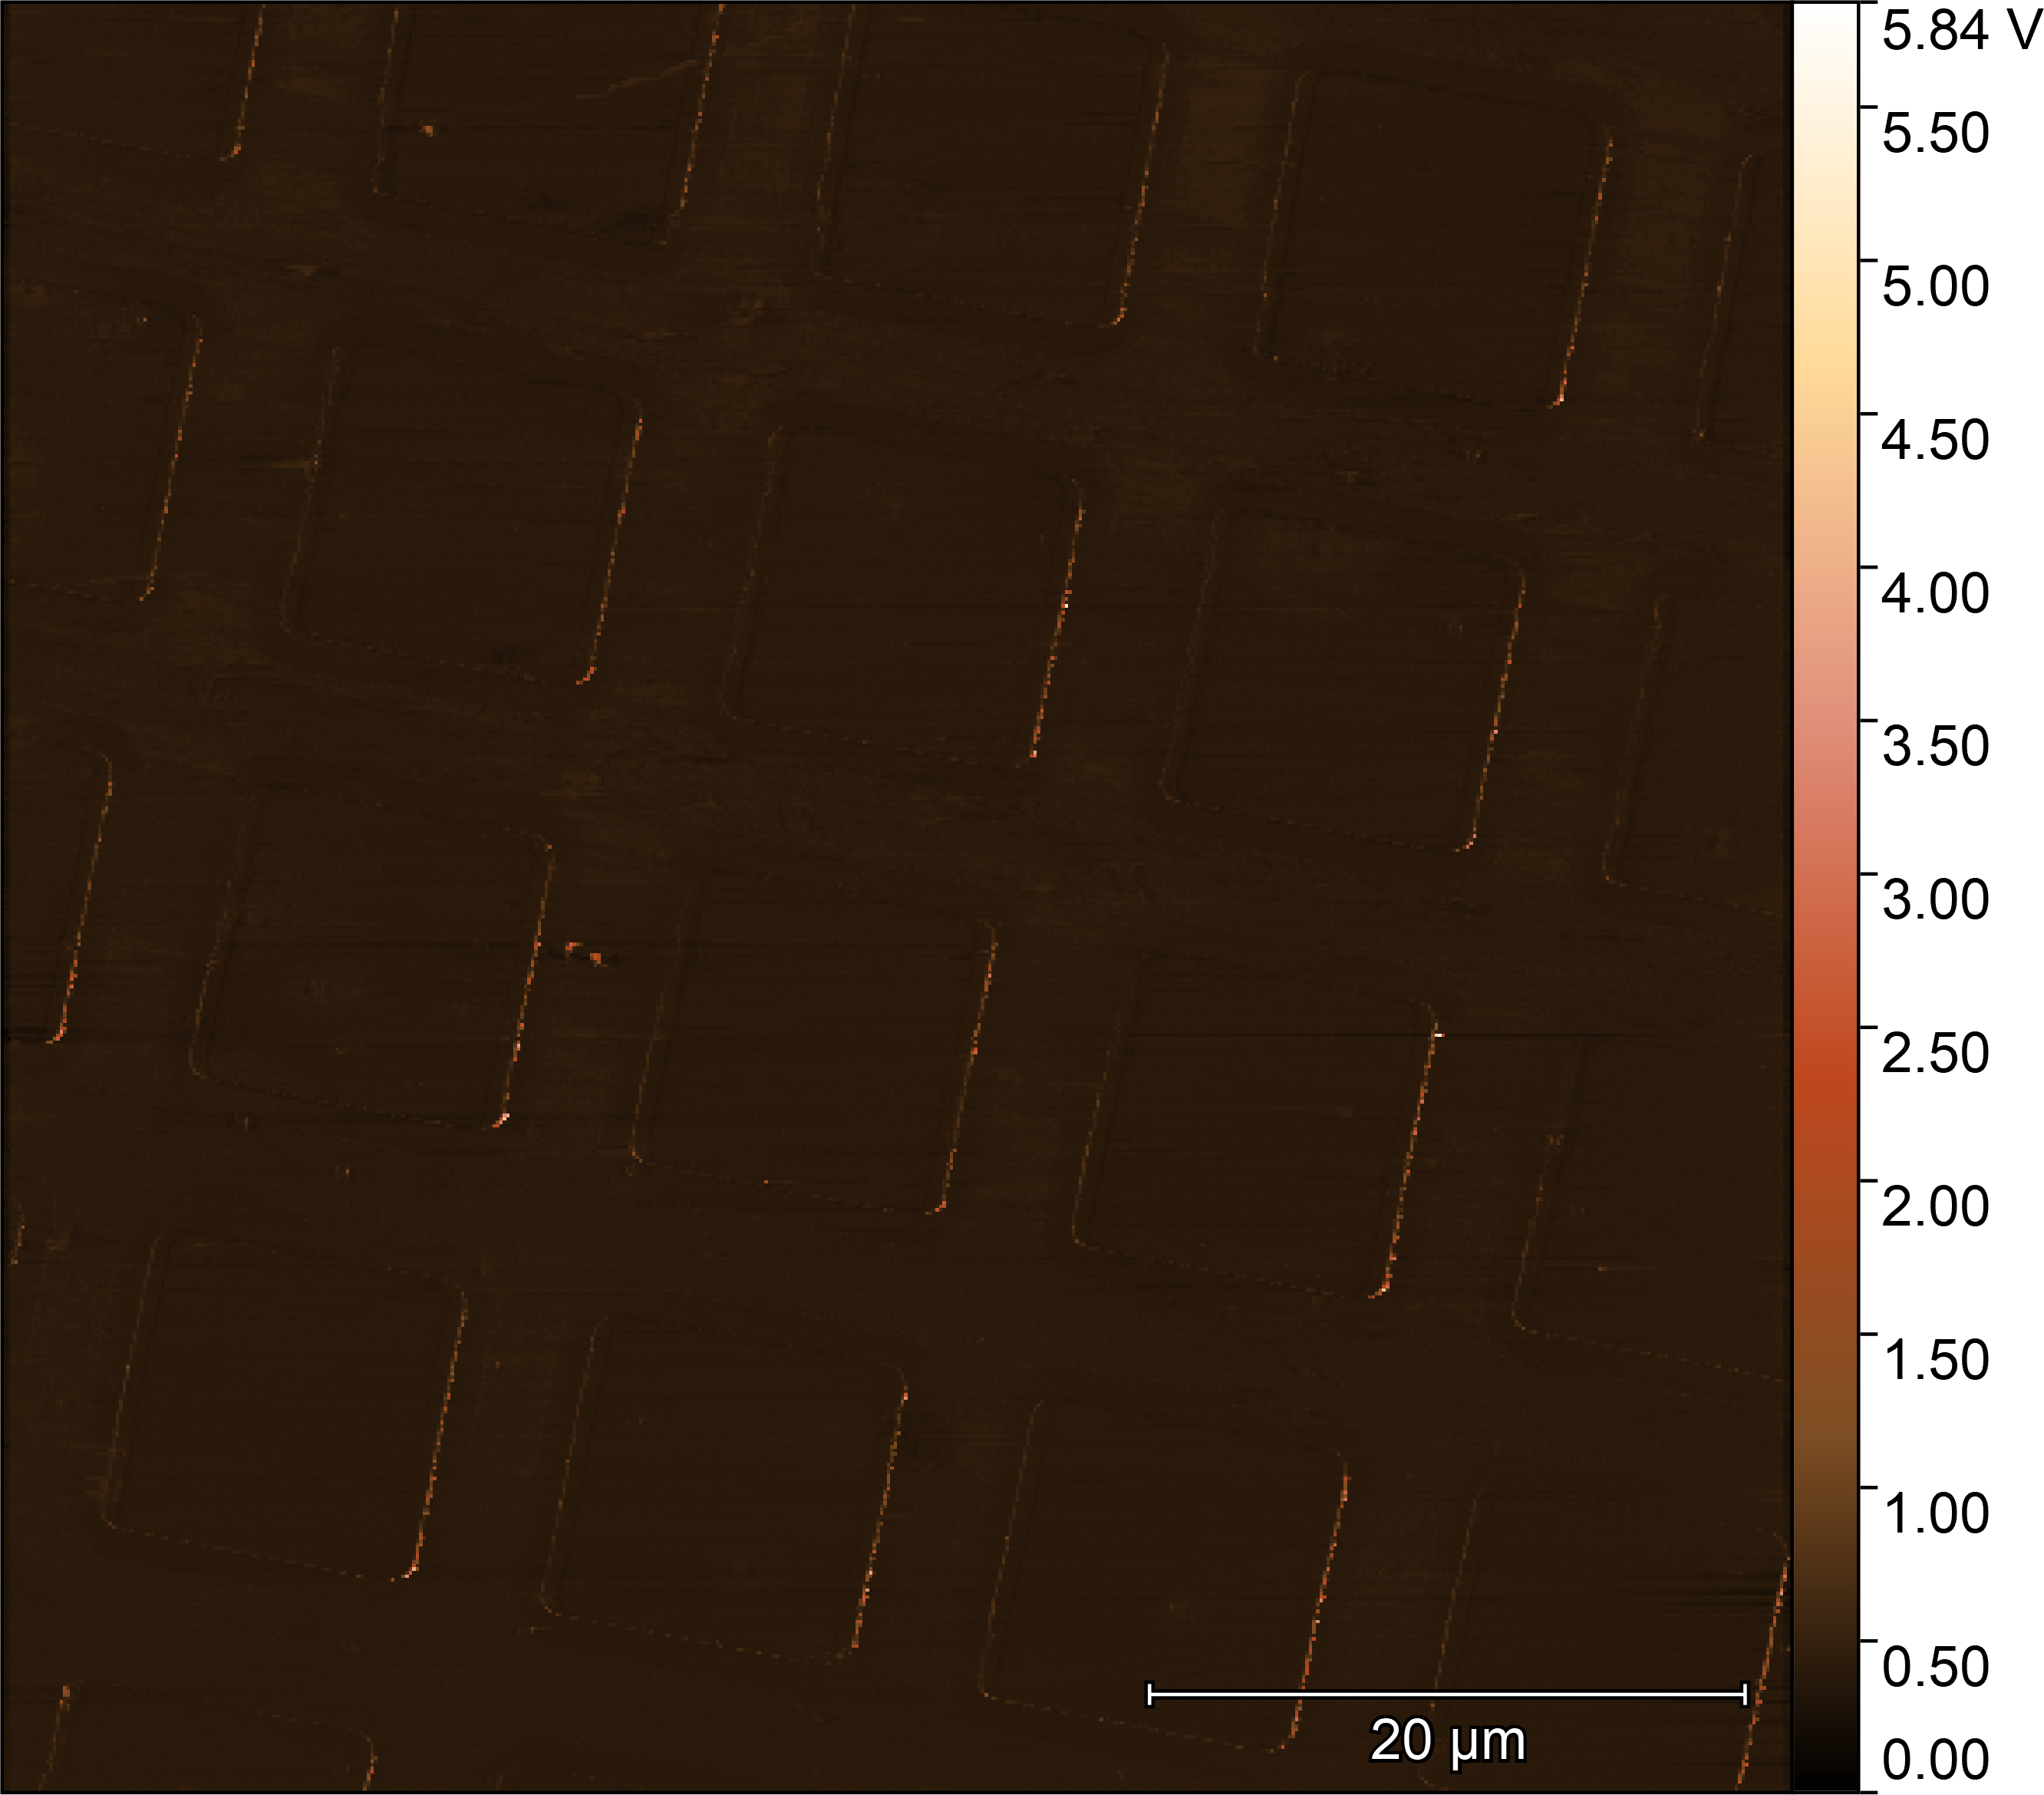
\includegraphics[width=.4\textwidth]{siatka_tarcie.png}
    \caption{Sygnał tarcia dla siatki kalibracyjnej}
    \label{fig:siatka_tarcie}
  \end{figure}

  \section{Topografia matrycy CCD}
  \begin{figure}[H]
    \centering
    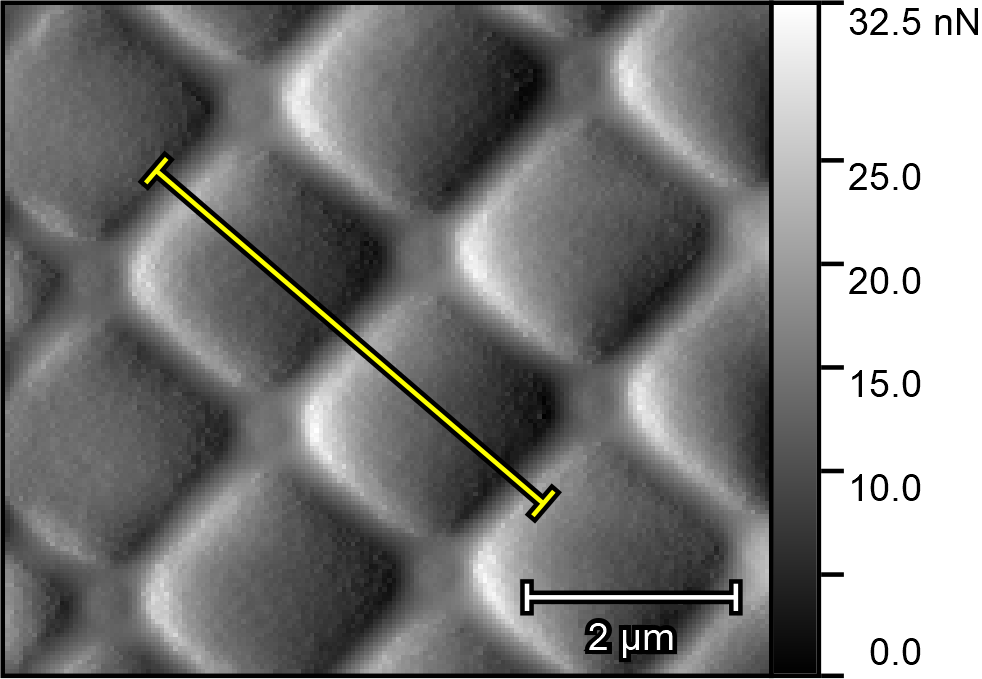
\includegraphics[width=.4\textwidth]{ccd_topo.png}
    \caption{Topografia matrycy CCD}
    \label{fig:ccd_topo}
  \end{figure}
  \begin{figure}[H]
    \centering
    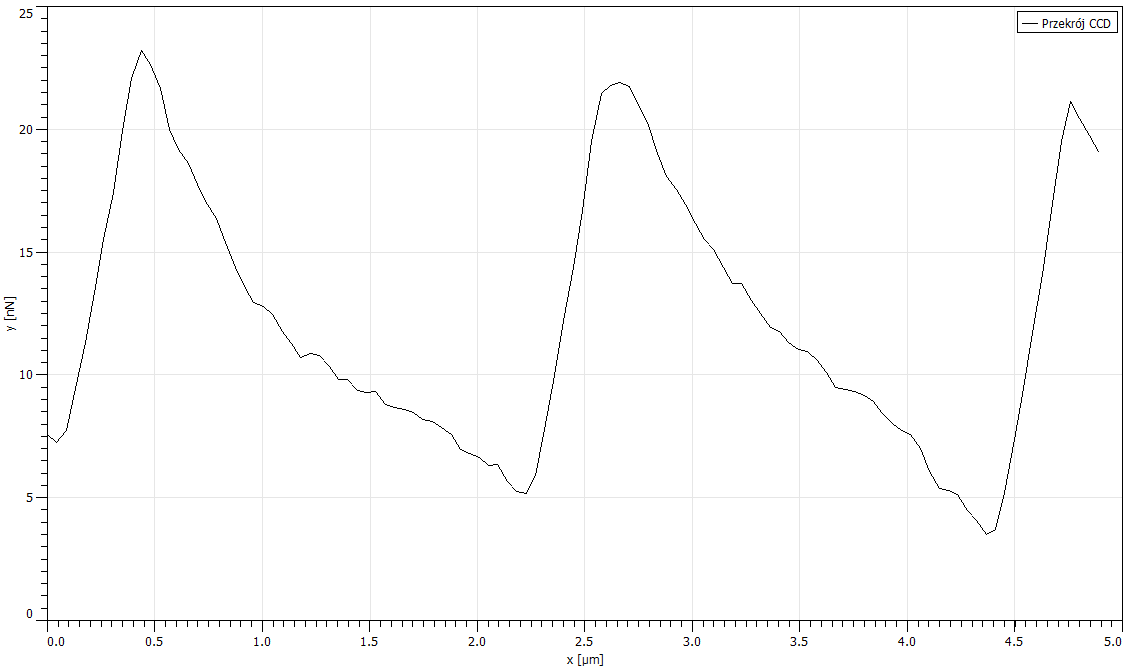
\includegraphics[width=.4\textwidth]{ccd_przekroj.png}
    \caption{Przekrój topografii matrycy CCD}
    \label{fig:ccd_przekroj}
  \end{figure}

  \clearpage

  \section{Topografia rGo}
  \begin{figure}[H]
    \centering
    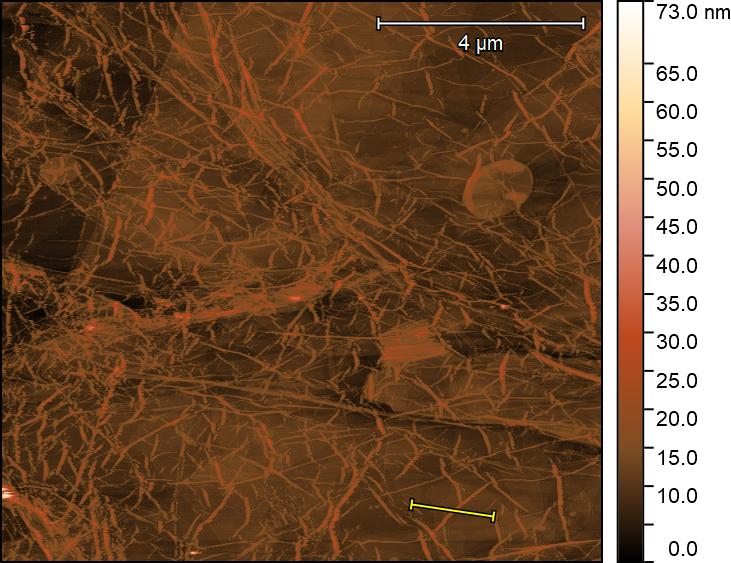
\includegraphics[width=.4\textwidth]{rgo_topo.png}
    \caption{Topografia rGo}
    \label{fig:rgo_topo}
  \end{figure}
  \begin{figure}[H]
    \centering
    \includegraphics[width=.4\textwidth]{rGo_przekroj.png}
    \caption{Przekrój topografii rGo}
    \label{fig:rGo_przekroj}
  \end{figure}

  \clearpage
  \onecolumn
  \begin{thebibliography}{9}
    \addcontentsline{toc}{section}{Bibliografia}
        
    \bibitem{binnig}
    Feynman Richard P., Leighton Robert B., Matthew Sands\\
    \textit{Feynmana wykłady z fizyki Tom I}

    \bibitem{davinci}
    Hutchings, Ian M.
    \textit{Leonardo da Vinci's studies of friction}
  \end{thebibliography}
\end{document}